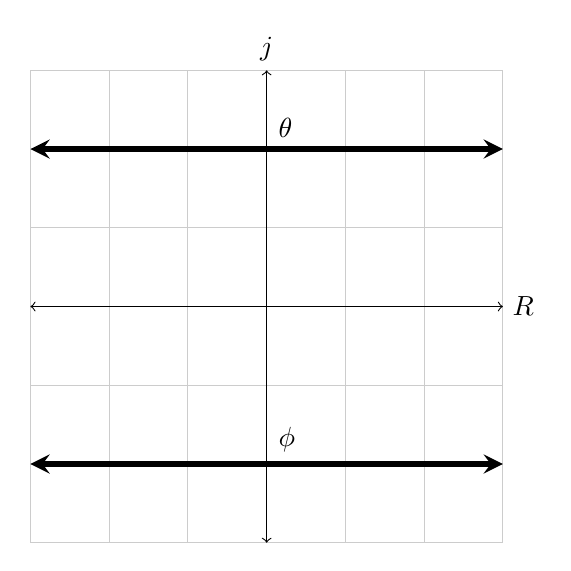
\begin{tikzpicture}
    \draw[thin,gray!40] (-3,-3) grid (3,3);
    \draw[<->] (-3,0)--(3,0) node[right] {$R$};
    \draw[<->] (0,-3)--(0,3) node[above]{$j$};
    
    \draw[line width=2pt,black,stealth-stealth] (-3,2)--(3,2)  node [midway,anchor=south west]{$\theta$};
    \draw[line width=2pt,black,stealth-stealth] (-3,-2)--(3,-2) node [midway,anchor=south west]{$\phi$};
\end{tikzpicture}
\caption*{Plano $w$}